\section{Introduction}

\subsection{Antibiotic resistance}

Antibiotics add, on average, twenty years to a person's life\cite{davies2013drugs}. However, antibiotic resistance is increasing alarmingly and is now recognised as a major threat to global health\cite{ResistanceUS,davies2013drugs}. Antibiotic discovery had its heyday in the 1940s to 60s, which saw the discovery of many new classes of antibiotic. Since then, the rate of discovery of new classes has slowed and resistance to existing treatments has increased.

The story of how Alexander Fleming discovered penicillin by accidentally allowing a Petri dish containing \textit{Staphylococcus aureus} to become contaminated with \textit{Penicillium} mould whilst he was on holiday in Suffolk \cite{davies2013drugs} is well known to many scientists. The initial serendipitous discovery of penicillin occurred in 1928 and was reported in 1929\cite{Fleming1929}, but it was not until 1943 that the drug was mass produced thanks to the research of Ernst Chain and Howard Florey. Unfortunately, bacterial resistance to penicillin was being found in hospitals by the late 1940s \cite{Barber1947, Rountree1949}. This alarmingly quick emergence of resistance is a common phenomenon for antibiotics (see \ref{tbl:AB_timeline}) as bacteria have multiple resistance mechanisms against antibacterial agents. These mechanisms can be broken down into five main categories\cite{ANIE:ANIE201209979,davies2013drugs}:

\begin{enumerate}
\item The bacterium may inactivate the drug before it can cause damage, for example the hydrolysis of $\beta$-lactam antibiotics such as penicillin by $\beta$-lactamase enzymes.

\item The bacterium may produce a membrane, cell wall or biofilm which does not allow the drug to pass through, for example biofilm formation may allow bacterial resistance to antibiotics to increase 1000-fold compared with bacteria in suspension culture\cite{Stewart2001}.

\item The bacterium may pump antibacterial molecules out of its cell membrane using efflux pumps, for example the mexAB and mexXY pumps used by \textit{Pseudomonas aeruginosa}\cite{Poole2004}.

\item Mutations may cause the target of the antibacterial molecule to alter such that the molecule no longer effectively binds the target, for example the alteration of penicillin binding proteins which are involved in the final stages of peptidoglycan biosynthesis in the cell walls of MRSA and other penicillin-resistant bacteria\cite{Fuda2004}.

\item The bacterium may switch to using a metabolic pathway which does not involve the target of the anti\hyp{}bacterial molecule, for example sulfonamide resistance may be achieved by taking in folic acid from the environment rather than synthesising it using \textit{para}-aminobenzoic acid - a process which is blocked by sulfonamides\cite{Skold2000}.

\end{enumerate}

\begin{table}[H]
  \centering
\begin{tabular}{|p{0.15\textwidth}|p{0.13\textwidth}|p{0.11\textwidth}|}
\hline  
\textbf{Antibiotic} & \textbf{Introduction} & \textbf{Resistance} \\ 
\hline
Sulfonamides & 1930s & 1940s \\ 
\hline 
Penicillin & 1943 & 1946 \\ 
\hline 
Streptomycin & 1943 & 1959 \\ 
\hline 
Chloramphenicol & 1947 & 1959 \\ 
\hline 
Tetracycline & 1948 & 1953 \\ 
\hline 
Erythromycin & 1952 & 1988 \\ 
\hline 
Vancomycin & 1956 & 1988 \\ 
\hline 
Methicillin & 1960 & 1961 \\ 
\hline 
Ampicillin & 1961 & 1973 \\ 
\hline 
Trimethoprim & 1962 & 1972 \\
\hline 
Cephalosporins & 1960s & late 1960s \\
\hline 
Ciprofloxacin & 1987 & 1988 \\
\hline 
Linezolid & 2000 & 1997 \\
\hline
Daptomycin & 2003 & 2005\\
\hline
\end{tabular}
\caption{A timeline of when various antibiotics were first introduced and when resistance to them first appeared\cite{Clatworthy2007,Palumbi2001,Ogle1988,Huovinen2001,Birmingham2003,Lee2007}.\label{tbl:AB_timeline}} 
\end{table}

The current pipeline of new antibiotics is widely thought to be worryingly inadequate\cite{Boucher2009,WHO,WEF}. Significant changes in how we use the antibiotics we already have, as well as investments in the discovery of new ones, are required.
Antibiotics currently in late-stage clinical trials nearly all rely on non-novel mechanisms of action\cite{Boucher2009}, and so it is almost inevitable that resistance to them will develop quickly, as it has done for their predecessors.

There is therefore increasing interest in treatments which would not easily provoke the development of resistance\cite{Spellberg2013}. These treatments often target bacterial virulence rather than killing bacteria outright, hence decreasing selection pressure for resistance\cite{Clatworthy2007}. 
One obvious target is toxin production, for example, an LpxC inhibitor was shown to prevent lethal \textit{Acinetobacter baumannii} infection in mice, despite being inactive against the bacterium \textit{in vitro}\cite{Lin2012}. This was due to inhibition of lipopolysaccharide shedding, and hence reduced inflammation in the host.
Co-ordination of virulence has also been targeted, for example, analogues of \textit{P. aeruginosa} homoserine lactone autoinducers (see \ref{sec:QS}) inhibit the production of virulence factors and increase the survival time of mice in a lethal \textit{P. aeruginosa} lung infection model\cite{Clatworthy2007}.

A second strategy in novel antibiotic discovery is to enhance or restore activity of a known antibiotic by lessening or avoiding a resistance mechanism. For example, antibiotics are often excluded from cells due to membrane impermeability or efflux. This may be overcome by attaching the antibiotic warhead to a molecule which the cell imports. The most well known examples of such conjugates are antibody-drug conjugates\cite{Lambert2018} in the treatment of cancer, but progress has also made against bacteria. In particular, siderophore-antibiotic conjugates (see \ref{sec:sidABCs}) have been investigated in the hope of hijacking bacterial uptake mechanisms to import antibiotics\cite{Page2013}, and the autoinducer-antibiotic conjugates in this study may gain activity by avoiding efflux pumps (see \ref{sec:AIABs}). These conjugates may have competing mechanisms of action: either the antibiotic accumulates in the cell to a greater extent and acts by its usual mechanism, or an important bacterial system must be disrupted to avoid accumulation of the antibiotic, hence leading to decreased fitness and/or loss of virulence.

\subsection{Siderophore-antibiotic conjugates\label{sec:sidABCs}}

Siderophore-antibiotic conjugates have been receiving attention in recent years as a way to enhance the uptake of known antibiotics\cite{Page2013}. This section will discuss the role of siderophores, sideromycins (natural siderophore-antibiotic conjugates), and the synthetic siderophore-antibiotic conjugates inspired by them. Many of the observations made about these molecules could be relevant to the autoinducer-antibiotic conjugates synthesised in this study.

\subsubsection{Siderophores}

Siderophores are peptides or small molecules used by microorganisms to chelate iron for the purposes of `iron mining'\cite{Hider2010}. Soluble iron is often scarce but it is crucial for many cellular processes including respiration and DNA synthesis. Siderophores are synthesised by the microorganisms and secreted into the extracellular environment where they bind to Fe$^{3+}$, often with exceptionally high affinities. The iron-bound siderophores are then brought back into the cell by active transport and the iron is released, either by reduction of the Fe$^{3+}$ to Fe$^{2+}$ or by enzymatic degradation of the siderophore. Siderophores have a wide range of structures (see \ref{fgr:Sids} and \ref{fgr:Sids_2}), possibly so one species can avoid its siderophores being taken up by another species\cite{Seyedsayamdost2012}.

\begin{figure}[H]
	\begin{center}
		\schemeref[ferri]{cmpd:ferri}
		\schemeref[fusar]{cmpd:fusar}
		\schemeref[defro]{cmpd:defro}
		\schemeref[rhodo]{cmpd:rhodo}
		\schemeref[yersin]{cmpd:yersin}
		\schemeref[entero]{cmpd:entero}
		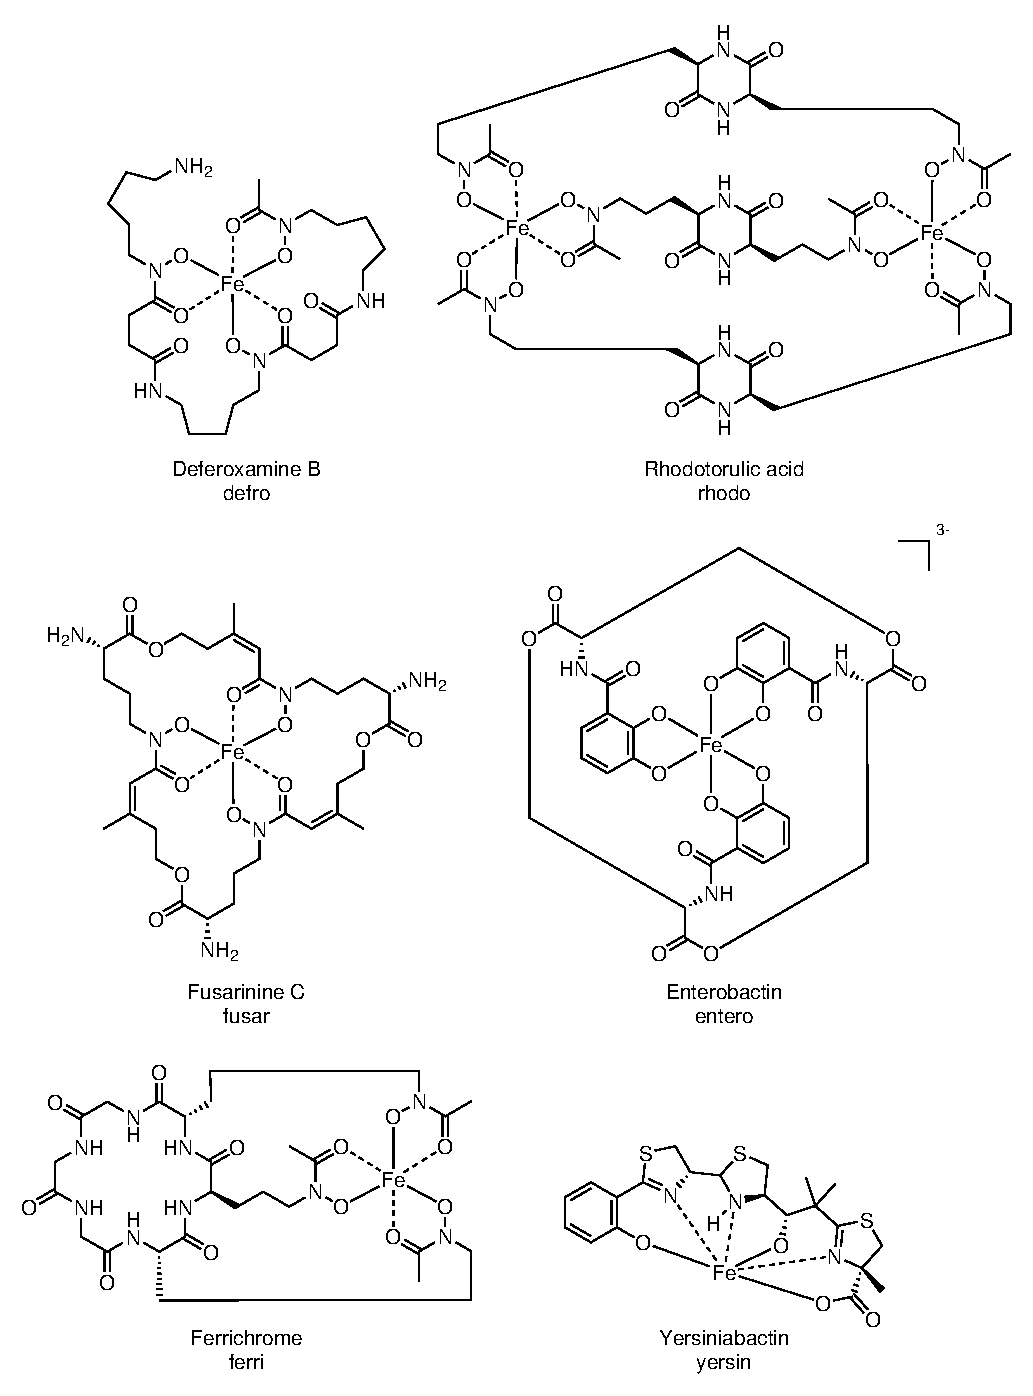
\includegraphics[scale=1]{Siderophores_1}
		\caption{Iron-siderophore complexes:
		Deferoxamine B \compound{cmpd:defro}\cite{Zheng2012} (\textit{Streptomyces pilosus} and \textit{Streptomyces coelicolor}), 
		rhodotorulic acid \compound{cmpd:rhodo}\cite{Carrano1978} (\textit{Rhodotorula pilimanae}),
		fusarinine C \compound{cmpd:fusar}\cite{Hossain1980} (\textit{Fusarium roseum}),
		enterobactin \compound{cmpd:entero}\cite{Zheng2012} (\textit{Escherichia coli} and enteric bacteria),
		ferrichrome \compound{cmpd:ferri}\cite{vanderHelm1980} (\textit{Ustilago sphaerogena}, \textit{U. maydis}, \textit{Aspergillus niger}, \textit{A. quadricintus}, \textit{A. duricaulis} and \textit{Penicillium resticolosum}),
		yersiniabactin \compound{cmpd:yersin}\cite{Zheng2012} (\textit{Yersinia pestis}).
		\label{fgr:Sids}}
	\end{center}
\end{figure}

\begin{figure}[H]
	\begin{center}
		\schemeref[pyo]{cmpd:pyov}
		\schemeref[pyoch]{cmpd:pyoch}
		
\includegraphics[scale=1]{Siderophores_2}
		\caption{Iron-siderophore complexes:
		pyoverdine PaA \compound{cmpd:pyov}\cite{Zheng2012,Meyer2000} (\textit{P. aeruginosa}, PAO1 strain) and pyochelin \compound{cmpd:pyoch}\cite{Schlegel2006,Cobessi2005} (\textit{P. aeruginosa}). 
		Note that pyochelin \compound{cmpd:pyoch} is a tetradentate ligand, hence the iron ion has two sites which can bind other ligands. \label{fgr:Sids_2}}
	\end{center}
\end{figure}

\subsubsection{Sideromycins}

Siderophore-antibiotic conjugates are produced naturally by some bacteria and are known as sideromycins\cite{Page2013} (see \ref{fgr:SidMys}). Bacteria produce these molecules to attack other bacteria by hijacking their siderophore uptake mechanisms to introduce toxic compounds. 

For example, albomycin \compound{cmpd:albo} (see \ref{fgr:SidMys}) is a sideromycin produced by \textit{Actinomyces subtropicus} and \textit{Streptomyces griseus}\cite{Hartmann1979,Fiedler1985} which has been used to treat infections caused by various bacteria including \textit{Yersinia enterocolitica} and \textit{Streptococcus pneumoniae} in mice and humans\cite{Gause1955,Pramanik2007}. 
Albomycin \compound{cmpd:albo} contains a siderophore coupled to a nuceloside antibiotic via a peptide linker. 
The siderophore section is structurally similar to ferrichrome \compound{cmpd:ferri} (see \ref{fgr:Sids}), a siderophore produced by various fungi, but also taken up by bacteria including \textit{Escherichia coli}, \textit{Salmonella typhimurium} and \textit{P. aeruginosa}\cite{vanderHelm1980,Hannauer2010}.
It has been shown that because of the structural similarity to ferrichrome \compound{cmpd:ferri}, \textit{E. coli} will also take up albomycin \compound{cmpd:albo}\cite{Hartmann1979}.
The linker is hydrolysed in the cytoplasm of the \textit{E. coli}, releasing the active nuceloside antibiotic. This leads to 500-fold concentration of the antibiotic within the \textit{E. coli} cells, enough to have significant effect on growth.

The success of albomycin\cite{Gause1955} and other sideromycins such as salmycin A\cite{Hider2010,Vertesy1995,Braun2009} and ferrimycin A1\cite{Sackmann1962,Gottlieb2012} has served as encouragement to many researchers to explore synthetic siderophore-antibiotic conjugates, which will be discussed in the next section. 

%Albomycin kills in vitro: staphylococci, Escherichia coli, Aerobacter aerogenes,Sarcina subflava, and Bacillus subtilis (Gause and Brazhnikova, 1951). Further, pneumococci, Klebsiella, dysentery bacilli, and some (but not all) strains of Streptococcus pyogenes are very sensitive. 

\begin{figure}[H]
	\begin{center}
		\schemeref[albo]{cmpd:albo}
		\schemeref[ferrim]{cmpd:ferrim}
		\schemeref[sal]{cmpd:sal}
		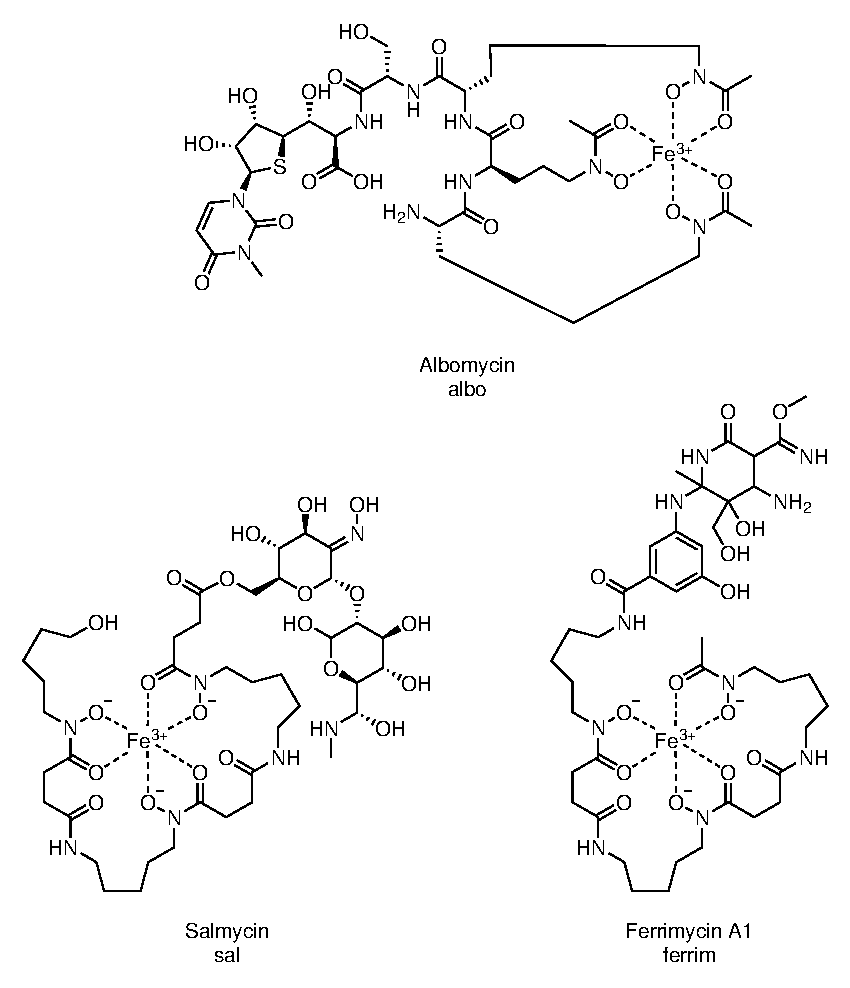
\includegraphics[scale=1]{SidMys}
		\caption{Iron-sideromycin complexes: Albomycin \compound{cmpd:albo}\cite{Benz1982,Hider2010} (\textit{Actinomyces subtropicus} and \textit{Streptomyces griseus}), salmycin A\cite{Hider2010,Vertesy1995,Braun2009} (\textit{Streptomyces violaceus}) and ferrimycin\cite{Hider2010} (\textit{Streptomyces griseoflavus}). \label{fgr:SidMys}}
	\end{center}
\end{figure}

\subsubsection{Synthetic siderophore-antibiotic conjugates\label{sec:synthsidABs}}

Sideromycins served as inspiration for the design, synthesis and biological evaluation of a wide range of synthetic siderophore-antibiotic conjugates\cite{Page2013}. Antibiotics used include $\beta$-lactams\cite{Mollmann2009,Dini2000,Kline2000}, nucleosides\cite{Lu1999}, glycopeptides\cite{Ghosh1996} and macrolides\cite{Ghosh1995}. Sideromycin-fluoroquinolone conjugates have also been studied by several groups\cite{Md-Saleh2009,Rivault2007,Ji2012}, including conjugates with linkers which can be cleaved\cite{Rivault2007,Ji2012} in a similar manner to albomycin\cite{Hartmann1979}. Some of these showed comparable activity to the parent antibiotic, but it is not clear whether attachment of the siderophore improved uptake or whether the conjugates acted as classical prodrugs.

$\beta$-lactam-sideromycin conjugates have been more widely investigated and show good activity \textit{in vitro}, however, resistance can evolve by loss of the TonB transporter or of the relevant siderophore receptor, e.g. Cir and Fiu for catecholate siderophores or FhuA for hydroxamate siderophores\cite{Page2013}. 
Recently a conjugate (Ent-Amp \compound{cmpd:Ent-Amp}, see \ref{fgr:synthsidABs}) of enterobactin and ampicillin joined using a copper(I)-catalyzed azide-alkyne cycloaddition has been shown to have increased activity against pathogenic \textit{E. coli} when compared to native ampicillin\cite{Zheng2014}. 
Other work has focused on monocyclic $\beta$-lactams, for example pirazmonam \compound{cmpd:Pir} and U-78608 \compound{cmpd:U-78}, which show high potency against Gram-negative bacteria including \textit{P. aeruginosa},\cite{Zurenko1990,Harrington2012}. Monocyclic $\beta$-lactams are generally fairly stable to $\beta$-lactamase activity, which is an advantage compared with many bicyclic $\beta$-lactams.

Three siderophore-antibiotic conjugates are reported as being in clinical trials\cite{Schalk2017}: MC-1 \compound{cmpd:MC-1}\cite{McPherson2012}, BAL30072 \compound{cmpd:BAL}\cite{Page2013} (see \ref{fgr:synthsidABs}) and cefiderocol \compound{cmpd:S-64}\cite{Ito2018,Saisho2018}.

MC-1 \compound{cmpd:MC-1} is reported as being `in clinical phases of development'\cite{Schalk2017}, but no reports of studies in humans could be found. However, experiments in mice have been promising\cite{McPherson2012}.
BAL30072 \compound{cmpd:BAL} is a siderophore-$\beta$-lactam conjugate which showed initial promise as it is a poor substrate for $\beta$-lactamases, and resistance due to loss of transport proteins is infrequent\cite{Page2013}. However, it is unclear whether it will progress further in trials as it causes liver toxicity\cite{Paech2017}. 
Cefiderocol \compound{cmpd:S-64} is a cephalosporin-catechol conjugate in phase 1 trials. Recent results indicate that `single and 35 multiple intravenous doses of cefiderocol at up to 2000 mg were well tolerated in healthy 36 subjects'\cite{Saisho2018}.

These examples show that siderophore-antibiotic conjugates are a promising strategy to deliver antibiotics across bacterial membranes, but it is worth noting that conjugation to a siderophore may lead to loss of activity, or resistance may be acquired by loss of transport proteins. Encouragingly though, albomycin \compound{cmpd:albo}-resistant mutants have been shown to be less virulent \cite{Pramanik2007}, indicating that bacteria may lose out either by susceptibility to the antibiotic or by loss of fitness due to decreased iron transport. 

Building on these positive examples, it is hoped that the strategy of conjugating a molecule which is important for virulence\cite{Vasil1999} with an antibiotic can be extended to conjugates of autoinducers and antibiotics in a similar `Trojan horse' approach.

\begin{figure}[H]
	\begin{center}
		\schemeref[bal]{cmpd:BAL}
		\schemeref[mc1]{cmpd:MC-1}
		\schemeref[ln]{cmpd:LN}
		\schemeref[s64]{cmpd:S-64}
		\schemeref[entamp]{cmpd:Ent-Amp}
		\schemeref[u78]{cmpd:U-78}
		\schemeref[pir]{cmpd:Pir}
		\includegraphics[scale=1]{sidABs}
		\caption{Examples of siderophore-antibiotic conjugates: Ent-Amp \compound{cmpd:Ent-Amp}\cite{Zheng2014}, 
		pirazmonam \compound{cmpd:Pir}\cite{Zurenko1990,Harrington2012}, 
		U-78608 \compound{cmpd:U-78},\cite{Zurenko1990,Harrington2012} 
		MC-1 \compound{cmpd:MC-1}\cite{McPherson2012},  
		BAL30072 \compound{cmpd:BAL}\cite{Page2013}
		and cefiderocol \compound{cmpd:S-64}\cite{Ito2018,Saisho2018}.
		\label{fgr:synthsidABs}}
	\end{center}
\end{figure}



\subsection{Autoinducer-antibiotic conjugates\label{sec:AIABs}}


This study extends the conjugation strategy discussed above by creating autoinducer-antibiotic conjugates. It was hypothesised that attaching an autoinducer to a known antibiotic could lead to increased cellular retention of the antibiotic, and could potentially restore function against resistant strains.
This section begins by introducing the concept of quorum sensing, followed by discussion of the autoinducers and antibiotics used in this study and the mechanisms of their efflux from \textit{P. aeruginosa} cells, and how these mechanisms could be exploited by conjugates.


\subsubsection{Quorum sensing\label{sec:QS}}

A quorum is defined as `A fixed minimum number of members of an assembly or society that must be present at any of its meetings to make the proceedings of that meeting valid.' \cite{Dictionary}  
A similar concept is used in bacterial signalling, whereby group behaviour is only triggered when a certain minimum concentration of bacteria has been reached. Examples of group behaviour include bioluminescence, the production of virulence factors, swarming and biofilm formation\cite{Miller2001}.  
It is advantageous for bacteria to coordinate such behaviours as they would be ineffective, and therefore a waste of resources, when carried out by a single bacterium.
The process by which bacteria determine the concentration of similar bacteria in their vicinity, and act on that information, is known as quorum sensing.

Quorum sensing has since been observed in many species of bacteria, including \textit{Vibrio fischeri}, \textit{P. aeruginosa}, \textit{Agrobacterium tumefaciens}, \textit{Erwinia carotovora}, \textit{Streptococcus pneumoniae}, \textit{Bacillus subtilis}, \textit{Staphylococcus aureus}, \textit{Vibrio harveyi}, \textit{Escherichia coli}, \textit{Myxococcus xanthus}, \textit{Salmonella enterica}, \textit{Yersinia enterocolitica}, \textit{Aeromonas sp.} and \textit{Acinetobacter sp.}\cite{Miller2001,Fuqua1994,Waters2005,Atkinson2006,Chan2011,Sauer2002,Michael2001,Ahmer2004,Nealson1970,Visick2006}. 
Many of these bacteria are significant causes of disease and death in humans, for example, in a typical year in the U.S. \textit{P. aeruginosa} causes 6,700 multidrug-resistant infections and 440 deaths, methicillin-resistant \textit{S. aureus} causes 80,500 severe infections and 11,300 deaths and non-typhoidal \textit{Salmonella} causes 1.2 million illnesses, 23,000
hospitalisations and 450 deaths\cite{ResistanceUS}.

\subsubsubsection{\textit{Vibrio fischeri}}

The first example of quorum sensing was discovered in \textit{V. fischeri}, a symbiotic bacterium that produces bioluminescence in the photophore of the Hawaiian bobtail squid, \textit{Euprymna scolopes} \cite{Nealson1970,Miller2001,Visick2006} (see \ref{fgr:ES}). This bacterium receives amino acids\cite{Graf1998, Lemus2000} from its host in exchange for producing light which the squid uses for counterillumination, to camouflage itself\cite{Jones2004}. 

If a low population of \textit{V. fischeri} were present in the photophore, the  light that the bacteria could produce would be insufficient to provide counterillumination. Therefore, the bacteria conserve resources by not producing light.
However, if there is a high population of \textit{V. fischeri} it is useful for them all to produce light, as this incentives the squid to provide them with nutrients. 


\begin{figure}[H]
	\begin{center}
		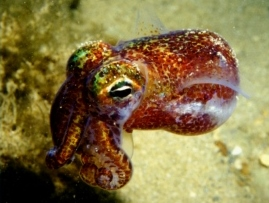
\includegraphics[height=5cm]{Euprymna_scolopes.jpg} 	
		\caption{`Euprymna scolopes, South shore of Oahu, Hawaii' by Jamie Foster. Licensed under CC BY-SA 3.0 via Commons.
		\label{fgr:ES}}
	\end{center}
\end{figure}


\textit{V. fischeri} uses the LuxR-LuxI system to sense cell density. This system is seen as a paradigm of quorum sensing, and a simplified explanation of it is presented to show typical features of such a system (see \ref{fgr:VFQS}).

\begin{figure}[H]
	\begin{center}
		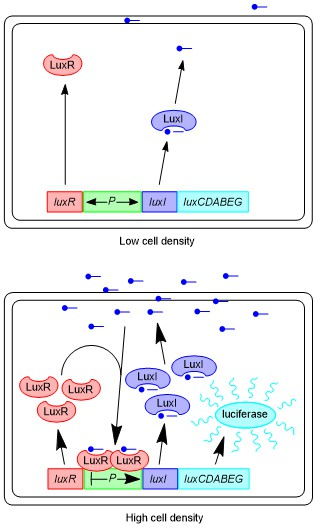
\includegraphics[width=0.5\textwidth]{VFQS}
		\caption{The LuxR-LuxI quorum sensing system in \textit{V. fischeri}. \label{fgr:VFQS}}
	\end{center}
\end{figure}


\textit{V. fischeri} senses cell concentration by the detection of 3-oxo-C$_6$-HSL \compound{cmpd:HLO6}\cite{Eberhard1981} (see \ref{fgr:HLO6}), a freely diffusible\cite{Kaplan1985} molecule which is synthesised by LuxI\cite{Parsek1999, Watson2002} and secreted by all \textit{V. fischeri} cells\cite{Schaefer1996} at a low basal level\cite{Miller2001}. 
When the bacterial population density, and hence the concentration of 3-oxo-C$_6$-HSL \compound{cmpd:HLO6}, reaches a threshold, 3-oxo-C$_6$-HSL \compound{cmpd:HLO6} binds to LuxR\cite{Hanzelka1995,Choi1991,Choi1992}, a receptor which is also synthesised at a low basal level. 

\begin{figure}[H]
	\begin{center}
		\schemeref[HLO6]{cmpd:HLO6}
		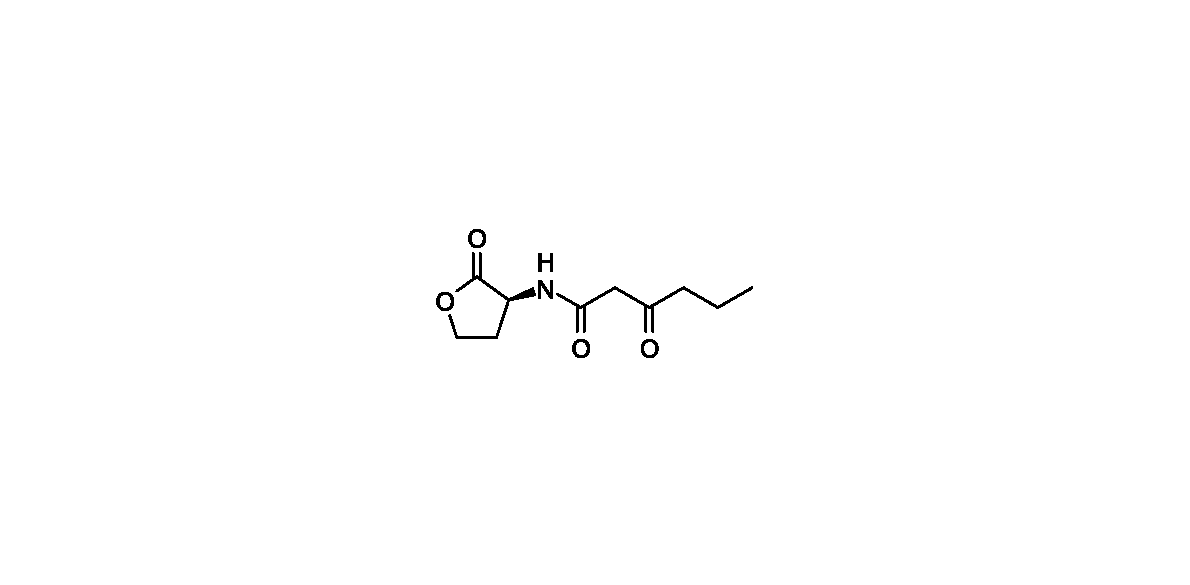
\includegraphics[scale=1]{HLO6.eps}
		\caption{3-oxo-C$_6$-HSL \compound{cmpd:HLO6}. \label{fgr:HLO6}}
	\end{center}
\end{figure}

The LuxR complex binds to the \textit{lux} operator, upregulating production of LuxI and hence 3-oxo-C$_6$-HSL \compound{cmpd:HLO6}, and luciferase enzymes and hence blue-green light\cite{Devine1989,Engebrecht1983,Visick2000}.
Production of more 3-oxo-C$_6$-HSL \compound{cmpd:HLO6} enables a positive feedback loop, reinforcing the effect of high population density on 3-oxo-C$_6$-HSL \compound{cmpd:HLO6} concentration and hence light production.
This is the reason that 3-oxo-C$_6$-HSL \compound{cmpd:HLO6} is known as an autoinducer.

The system also contains a negatively feedback loop to avoid excessive expression of proteins: at high concentrations of 3-oxo-C$_6$-HSL \compound{cmpd:HLO6} production of LuxR is inhibited\cite{Dunlap1989}. Such balancing effects, as well as interactions with other quorum sensing and metabolic systems, are very common.

\subsubsubsection{\textit{Pseudomonas aeruginosa}\label{sec:PA}}

Another well-studied example of quorum sensing is in \textit{P. aeruginosa}\cite{Dubern2008,Hodgkinson2011,Jimenez2012}.
\textit{P. aeruginosa} is a Gram-negative opportunistic pathogen which typically infects immunocompromised individuals such as those with cystic fibrosis, neutropenia and AIDS. It can infect the pulmonary and urinary tracts as well being the most frequent cause of burn wound infections and the most frequent conloniser of medical devices such as catheters\cite{Bodey1983}. Multidrug-resistant \textit{P. aeruginosa} is classified as a `serious threat' by the United States Centers for Disease Control and Prevention\cite{ResistanceUS} and carbapenem-resistant \textit{P. aeruginosa} is classified as `priority 1: critical' by the World Health Organisation\cite{WHO}.

\textit{P. aeruginosa} has a low susceptibility to many antibiotics and readily acquires antibiotic resistance by mutation or horizontal gene transfer\cite{Cornelis2008}.
It is difficult for antibiotics to cross into cells due to low cell membrane permeability\cite{Nikaido1989} and biofilm formation\cite{Evans1991}, and they are pumped out again by its multiple chromosomally encoded multidrug efflux pumps\cite{Poole2004}.
\textit{P. aeruginosa} biofilms are more resistant to many drugs including ciprofloxacin \compound{cmpd:Cip} and trimethoprim \compound{cmpd:Tri} compared with planktonic cells\cite{Evans1991,Olson2002}.
This high level of antibiotic resistance makes \textit{P. aeruginosa} an important target for drug discovery.

Quorum sensing in \textit{P. aeruginosa} involves a complex interplay of five signalling molecules (see \ref{fgr:PA_autoinducers}) and various proteins (see \ref{fgr:PA_QS})\cite{Dubern2008,Hodgkinson2011,Jimenez2012}.
These can be broken down into three main, interacting systems: Las, Rhl and Pqs.

\begin{figure}[H]
	\begin{center}
		\schemeref[HL4]{cmpd:HL4}
		\schemeref[HLO12]{cmpd:HLO12}
		\schemeref[PQS1]{cmpd:PQS}
		\schemeref[HHQ1]{cmpd:HHQ}
		\schemeref[AI2]{cmpd:AI2}
		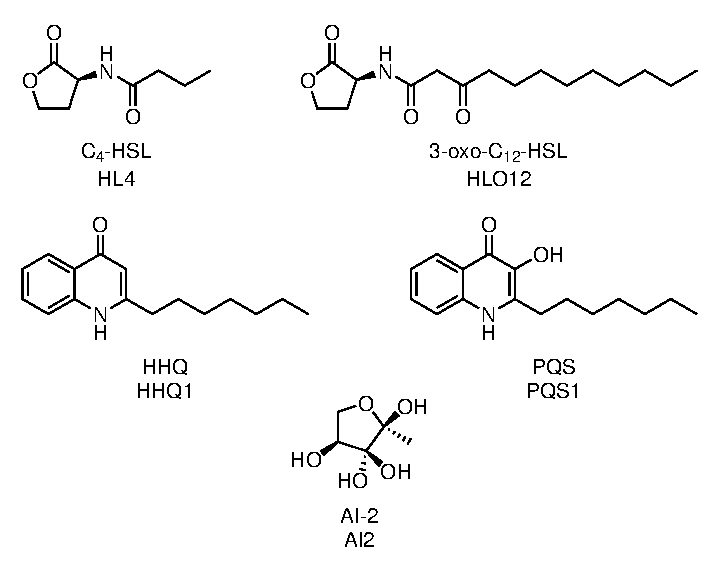
\includegraphics[scale=1]{PA_QSMs}
		\caption{\textit{P. aeruginosa} autoinducers. \label{fgr:PA_autoinducers}}
	\end{center}
\end{figure}

In the Las system, LasI\cite{Wargo2007} synthesises the 3-oxo-C$_{12}$-HSL \compound{cmpd:HLO12}\cite{Pearson1994} autoinducer. 
3-oxo-C$_{12}$-HSL \compound{cmpd:HLO12} binds LasR\cite{Gambello1991}, and this complex upregulates the production of LasI\cite{Pesci1997} (thus causing autoinduction) as well as 
alkaline protease\cite{Gambello1993}, elastase\cite{Gambello1991}, exotoxin A\cite{Gambello1993}, HCN\cite{Pessi2000} and LasA protease\cite{Toder1991}.
The LasR complex is also important in late-stage biofilm formation\cite{Sauer2002}, and upregulates the Rhl\cite{Latifi1996} and Pqs systems\cite{Gallagher2002,Wade2005}.

In the Rhl system, RhlI\cite{Brint1995} synthesises the C$_4$-HSL \compound{cmpd:HL4}\cite{Pearson1995} autoinducer. 
C$_4$-HSL \compound{cmpd:HL4} binds RhlR\cite{Winson1995}, and this complex upregulates the production of RhlI\cite{Pesci1997} (again causing autoinduction), 
alkaline protease\cite{Latifi1995}, elastase\cite{Brint1995}, haemolysin\cite{Latifi1995}, HCN\cite{Pessi2000,Latifi1995}, LasA protease\cite{Brint1995}, LecA\cite{Winzer2000}, pyocyanin\cite{Brint1995,Latifi1995} and rhamnolipids\cite{Brint1995}.
The RhlR complex also downregulates the Pqs system\cite{McGrath2004,Wade2005}.
The Rhl system is controlled by both the Las and Pqs systems,
as production of both RhlR and RhlI is upregulated by the LasR complex\cite{Latifi1996} 
and production of both RhlR is upregulated by the PqsR complex\cite{McKnight2000}.
%not biofilms\cite{Davies1998}


In the Pqs system, the main autoinducer, PQS \compound{cmpd:PQS}\cite{Pesci1999}, is synthesised by multiple enzymes. 
PhnAB\cite{Farrow2007}, PqsA, PqsBC, PqsD\cite{Lepine2003,Lepine2004} and PqsE\cite{Drees2015,Lin2018} produce the precursor HHQ \compound{cmpd:HHQ}, and PqsH converts HHQ \compound{cmpd:HHQ} to PQS \compound{cmpd:PQS}. 
PQS \compound{cmpd:PQS}\cite{Wade2005} or HHQ \compound{cmpd:HHQ} binds PqsR\cite{Xiao2006}, and either complex can upregulate the synthesis of HHQ \compound{cmpd:HHQ} causing autoinduction. 
The PqsR-PQS complex upregulates the production of 
chitinase\cite{Deziel2005}, elastase\cite{Pesci1999}, HCN\cite{Deziel2005}, LecA\cite{Diggle2003}, pyocyanin\cite{Gallagher2002,Diggle2007} and pyoverdine\cite{Diggle2007}, as well as increasing biofilm production\cite{Diggle2003} and vesicle formation\cite{Mashburn2009}.
The PqsR-PQS complex also upregulates production of RhlR, so the Pqs system has control over the Rhl system\cite{McKnight2000}.
The Pqs system is controlled by both the Las and Rhl systems,
as production of PqsR\cite{Wade2005} and PqsH\cite{Gallagher2002} is upregulated by the LasR complex and 
production of PqsA, PqsBC, PqsD, PqsE\cite{McGrath2004} and PqsR\cite{Wade2005} is downregulated by the RhlR complex.

\todo{add numbers manually when sorted}

\begin{figure}[H]
	\begin{center}
		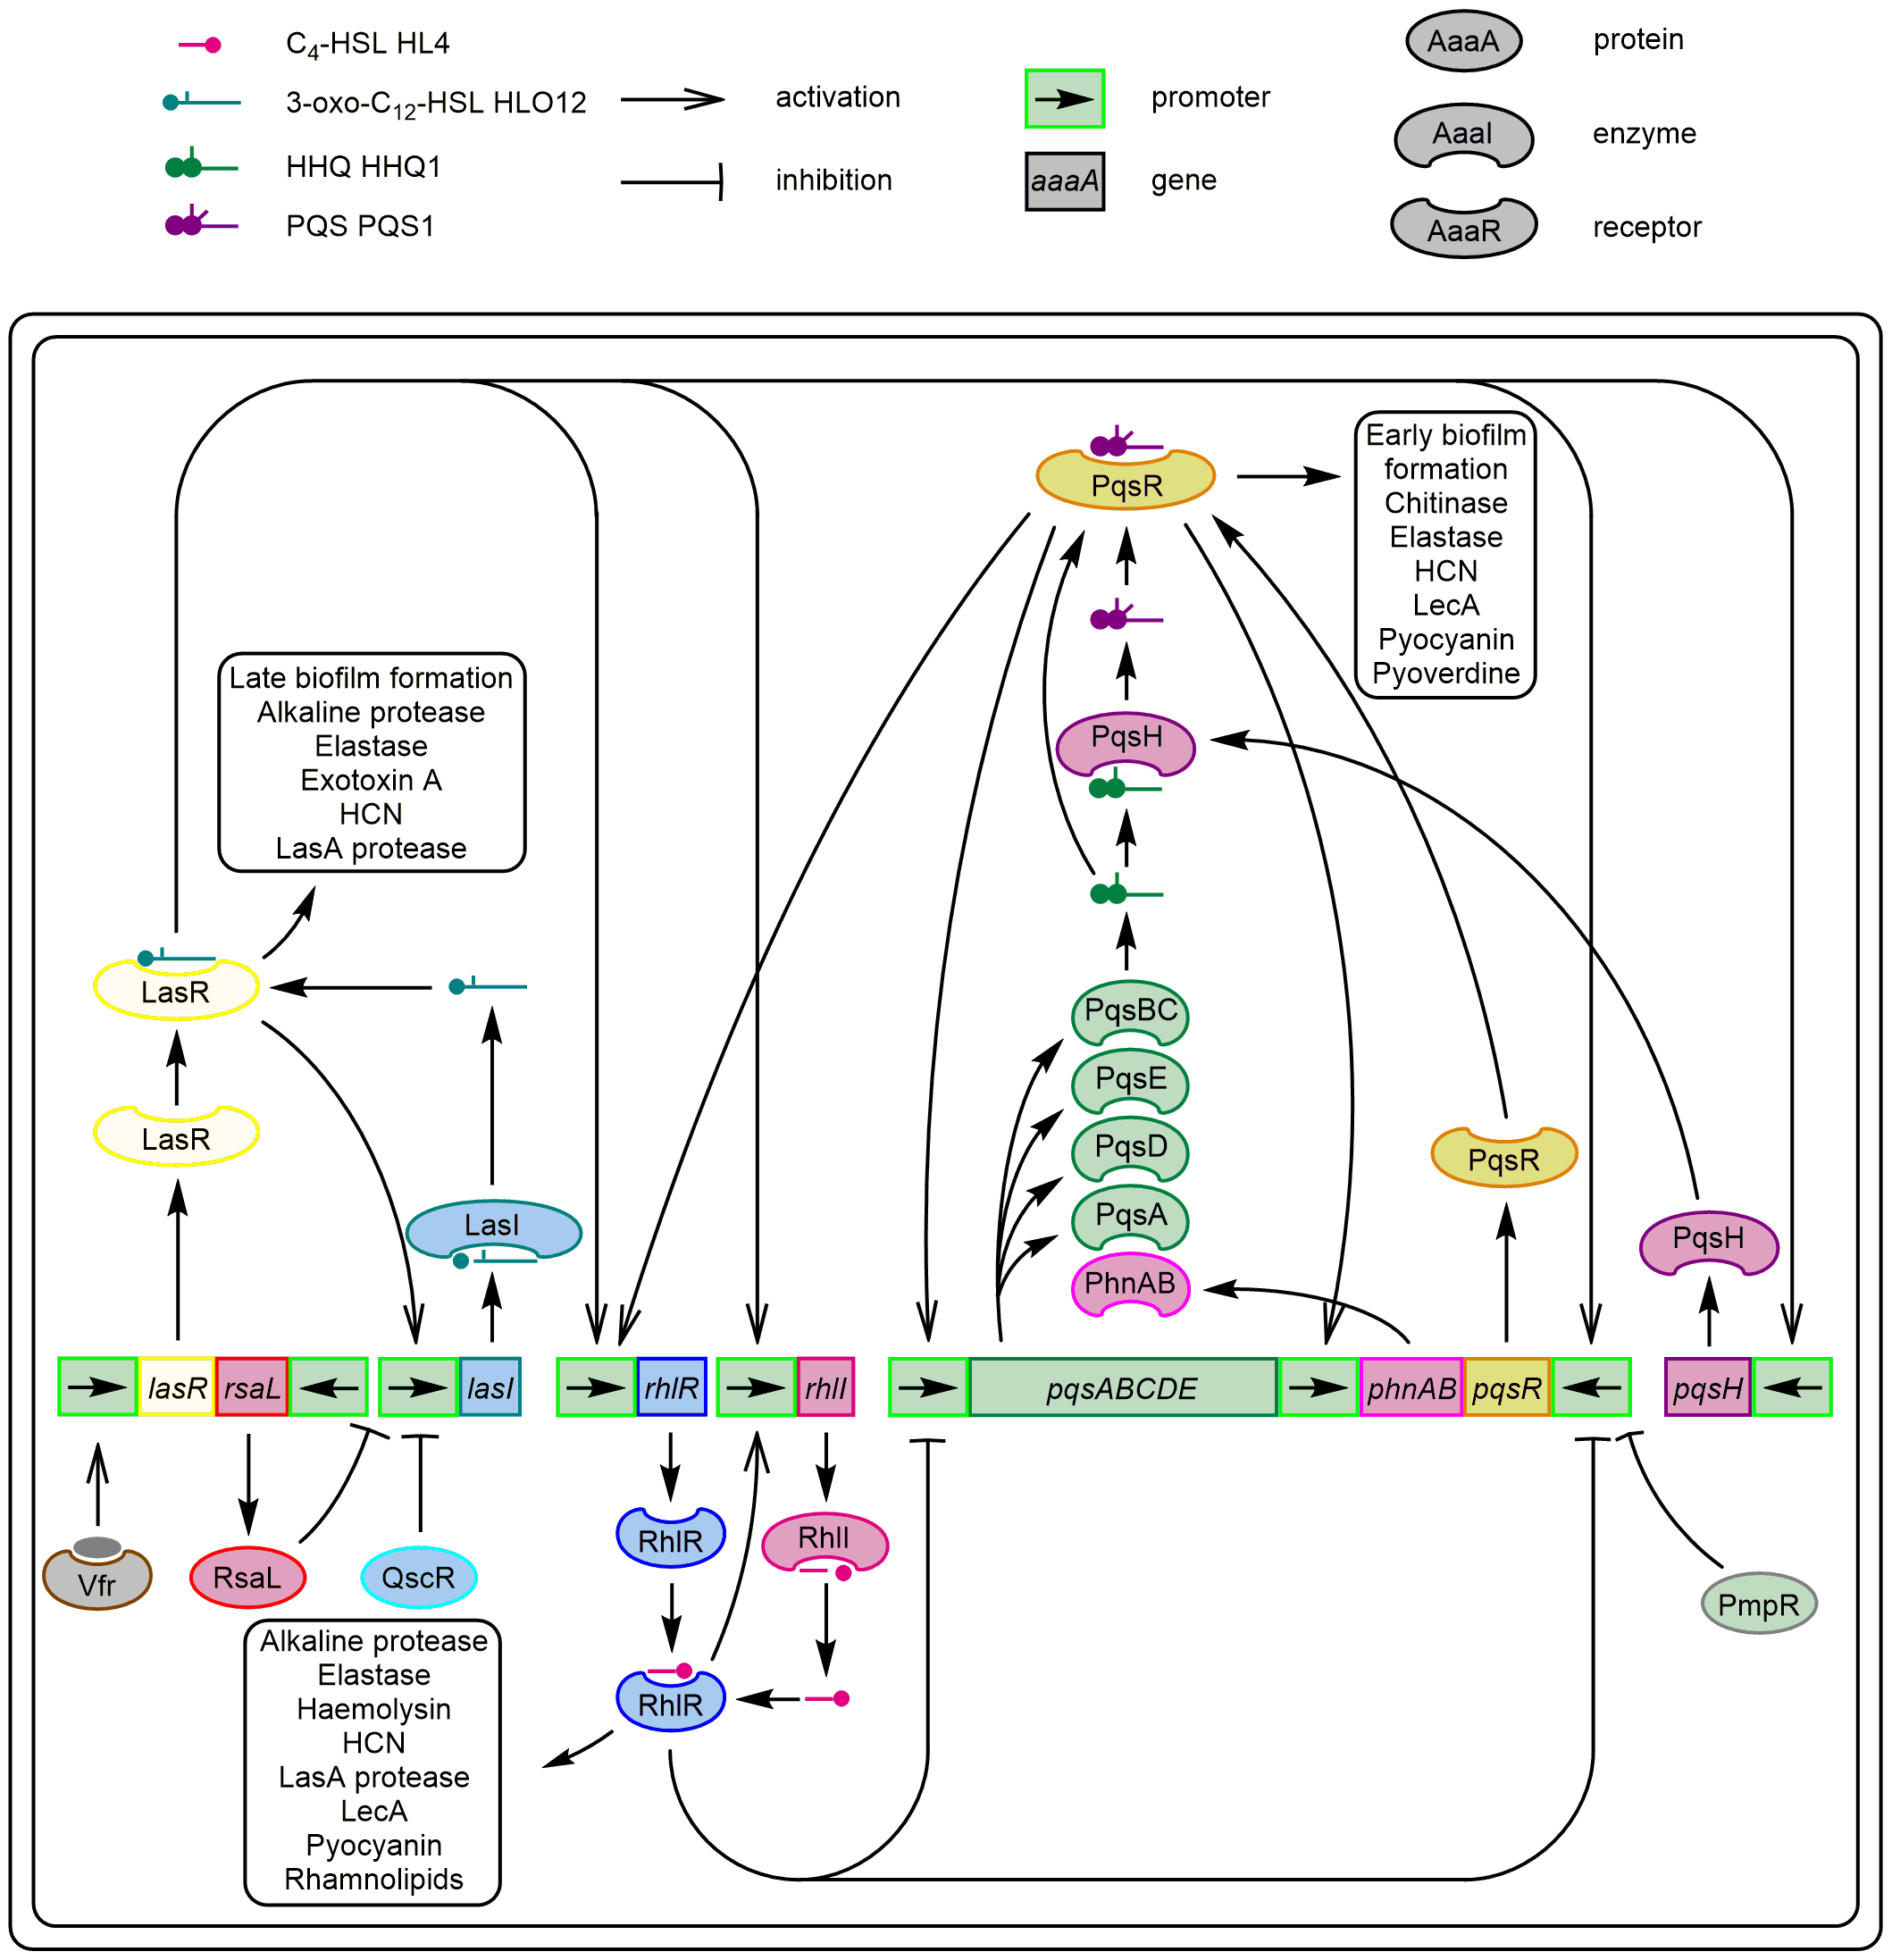
\includegraphics[width=\textwidth]{PAQS_full}
		\caption{Quorum sensing in \textit{P. aeruginosa}\cite{Dubern2008,Hodgkinson2011,Jimenez2012}. \label{fgr:PA_QS}}
	\end{center}
\end{figure}

%ideally save as tiff then convert to png

In addition to the above systems, AI-2 (see \ref{fgr:PA_autoinducers}), an interspecies signalling molecule\cite{Pereira2013}, is known to increase biofilm production and virulence in \textit{P. aeruginosa}\cite{Li2015a,Li2017}. This is thought to be achieved by interaction with the Las and Rhl systems, but the exact mechanism is not known.

In summary, \textit{P. aeruginosa} uses the autoinducers shown in \ref{fgr:PA_autoinducers} as part of three interacting quorum sensing systems to coordinate virulence and biofilm production, and this makes these autoinducers interesting therapeutic targets. 

%Rampioni RsaL inhibits HCN and pyocyanin
%%Vfr\cite{Albus1997}

\subsubsection{Autoinducers}

Quorum sensing has been sucessfully targeted using many different modulators\cite{Galloway2011,Hodgkinson2011}, but this study takes a slightly different approach. 
Inspired by the success of various siderophore-antibiotic conjugates (see \ref{sec:synthsidABs}), a library of autoinducer-antibiotic conjugates was synthesised, in the hope that the importance of autoinducers in harmful cellular behaviours would lead to increased activity of the conjugates (see \ref{sec:AIABs}).

The \textit{P. aeruginosa} autoinducers (see \ref{fgr:PA_autoinducers}) were chosen for use in this study as \textit{P. aeruginosa} is a significant human pathogen which shows high antibiotic resistance and utilises quorum sensing to coordinate pathogenic behaviours (see \ref{sec:PA}). 
Specifically, C$_4$-HSL \compound{cmpd:HL4}, HHQ \compound{cmpd:HHQ} and PQS \compound{cmpd:PQS} derivatives were chosen as they were considered to be the most synthetically tractable.

\subsubsection{Autoinducer efflux\label{sec:AI_eff}}

Autoinducers must be exported from the cell in order to be used for intercellular communication, and the five known \textit{P. aeruginosa} autoinducers are exported by various different transport mechanisms.
The mechanism is not well known for HHQ \compound{cmpd:HHQ} or AI-2 \compound{cmpd:AI2}, but it is know that
PQS \compound{cmpd:PQS} is exported in vesicles\cite{Florez2017},
C$_4$-HSL \compound{cmpd:HL4} passively diffuses in and out of cells\cite{Pearson1999}, and
3-oxo-C$_{12}$-HSL \compound{cmpd:HLO12} is taken up passively, accumulates in the cell membrane and is actively pumped out by efflux pumps.
The difference in transport mechanism for C$_4$-HSL \compound{cmpd:HL4} and 3-oxo-C$_{12}$-HSL \compound{cmpd:HLO12} is thought to be largely due to chain length rather than the 3-oxo modification, as a shorter-chain version, 3-oxo-C$_6$-HSL \compound{cmpd:HLO6} has been shown to be freely diffusable through \textit{V. fischeri} membranes\cite{Kaplan1985}.

3-oxo-C$_{12}$-HSL \compound{cmpd:HLO12} is exported primarily via the MexAB-OprM efflux system\cite{Evans1998,Poole2004}.
The increased removal of 3-oxo-C$_{12}$-HSL \compound{cmpd:HLO12} from the cell by upregulation of the MexAB-OprM system leads to decreased production of additional 3-oxo-C$_{12}$-HSL \compound{cmpd:HLO12} (as the positive feedback loop is disrupted, see \ref{sec:PA}), and hence decreased production of pyocyanin, elastase and casein protease. 
It is expected that MexAB-OprM upregulation would also disrupt biofilm formation as a decrease in 3-oxo-C$_{12}$-HSL \compound{cmpd:HLO12} levels would disrupt Las-mediated quorum sensing\cite{Davies1998}, but no direct studies of this could be found.

\subsubsection{Antibiotics}

Ciprofloxacin \compound{cmpd:Cip} and trimethoprim \compound{cmpd:Tri} (see \ref{fgr:ABs}) were chosen as the antibiotic sides of the conjugates.
 
Ciprofloxacin \compound{cmpd:Cip} is second-generation fluoroquinolone antibiotic used to treat both Gram-positive and Gram-negative bacterial infections including \textit{P. aeruginosa}\cite{Oliphant2002,Macgowan1999}. Ciprofloxacin \compound{cmpd:Cip} inhibits DNA replication by binding to DNA gyrase and topoisomerase IV\cite{Drlica1997}.


Trimethoprim (see \ref{fgr:ABs}) is a dihydrofolate reductase inhibitor used primarily to treat bladder infections\cite{Brogden1982}. It is active against several significant human pathogens including \textit{Streptococcus pneumoniae} and \textit{Haemophilus influenzae}, but not against \textit{P. aeruginosa}. It was primarily chosen in this study as it was considered easy to functionalise, but also to test the feasibility of creating antibiotic activity against \textit{P. aeruginosa}.

\begin{figure}[H]
	\begin{center}
		\schemeref[Cip]{cmpd:Cip}
		\schemeref[Tri]{cmpd:Tri}
		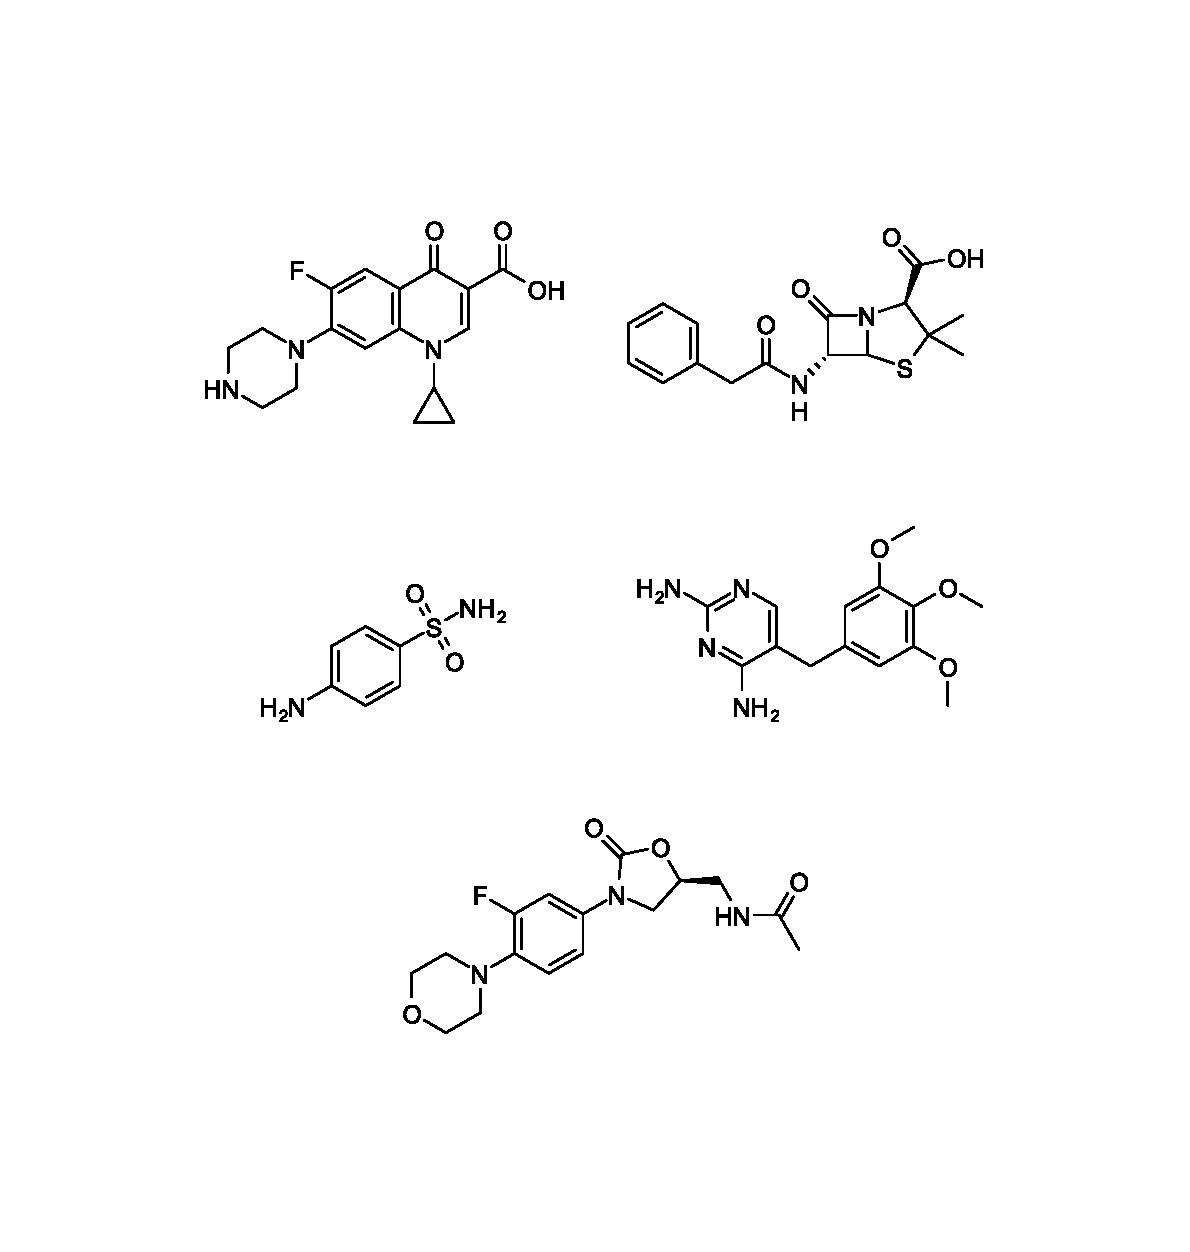
\includegraphics[scale=1]{ABs}
		\caption{The antibiotics used in this section. \label{fgr:ABs}}
	\end{center}
\end{figure}



\subsubsection{Antibiotic efflux}

Ciprofloxacin \compound{cmpd:Cip} enters \textit{P. aeruginosa} by diffusion\cite{Celesk1989}, but is pumped out by efflux pumps\cite{Poole2000}. In the planktonic state several efflux pumps are known to pump out ciprofloxacin \compound{cmpd:Cip}, including MexAB–OprM, MexCD–OprJ, MexEF–OprN, MexXY–OprM, MexJK–OprM and MexVW–OprM\cite{Poole2004}. 
However, in biofilms only MexEF-OprN has an effect\cite{DeKievit2001}.

Trimethoprim \compound{cmpd:Tri} is mainly exported by the MexAB–OprM\cite{Kohler1996}, MexCD–OprJ\cite{Poole1996} and MexEF–OprN\cite{Kohler1997} multidrug efflux systems\cite{Poole2001,Poole2004} in the planktonic state. It is not known which pumps are used to export trimethoprim \compound{cmpd:Tri} from biofilms, but biofilms do show increased resistance to it\cite{Olson2002}.

\subsubsection{Conjugate efflux and antibiotic action\label{sec:conj_eff}}

There are two ways in which the conjugates could disrupt \textit{P. aeruginosa} growth:

\begin{enumerate}

\item \textit{P. aeruginosa} could develop resistance to an autoinducer-antibiotic conjugate by upregulation of its export mechanism, but this would also lead to increased export of the native autoinducer, thus disrupting the quorum sensing system and hence biofilm formation and virulence\cite{Dubern2008,Davies1998,Evans1998}.
For HSL conjugates this would mean upregulation of the MexAB-OprM pump, as this is the pump used for export of 3-oxo-C$_{12}$-HSL \compound{cmpd:HLO12}\cite{Evans1998,Poole2004}.
For PQS conjugates this would mean upregulation of vesicle formation\cite{Florez2017}.

\item The autoinducer section could make the conjugate a poor substrate for the antibiotic section's usual efflux mechanism, leading to accumulation of the conjugate within cells and hence increased antibacterial activity. 
For autoinducer-ciprofloxacin conjugates acting on planktonic \textit{P. aeruginosa} this would mean the conjugate being a poor substrate of the various efflux pumps listed in the previous section.
For autoinducer-ciprofloxacin conjugates acting on biofilms this would mean the conjugate being a poor substrate of MexEF–OprN (the sole exporter of ciprofloxacin \compound{cmpd:Cip} in biofilms\cite{DeKievit2001} and not an exporter of HSLs \compound{cmpd:HL4} or \compound{cmpd:HLO12}, or PQS \compound{cmpd:PQS}\cite{Poole2004}).
This mechanism could in principal work for trimethoprim \compound{cmpd:Tri} as well, but it is not known which pumps are active against this antibiotic in biofilms. 

\end{enumerate}


These synergistic mechanisms of action made autoinducer-antibiotic conjugates a promising target. An initial library was designed using a copper(I)-catalysed azide-alkyne cycloaddition\cite{Tornoe2002,Rostovtsev2002}, commonly referred to as a click reaction (although this is a more general term), to join each combination of autoinducer and antibiotic together. 



\subsubsection{Cleavable linkers\label{sec:cleavable_intro}}

\todo{cleavable intro}

As part of the library, a set of cleavable HSL-ciprofloxacin triazole conjugates was synthesised in collaboration with Professor Eddy Sotelo.
These were based on the cleavable pyochelin–norfloxacin conjugates synthesised by Rivault \textit{et al.}\cite{Rivault2007} (see \ref{fgr:pyNors}).
The linker was chosen with the hope that it would be stable under the extracellular assay conditions, but would be cleaved upon entry into the cell by intracellular esterases. It was hoped that the attached HSLs would improve retention of the conjugate in cells. 

\begin{figure}[H]
	\begin{center}
		\schemeref[pyNor]{cmpd:pyNor}
		\schemeref[pyYNor]{cmpd:pyYNor}
		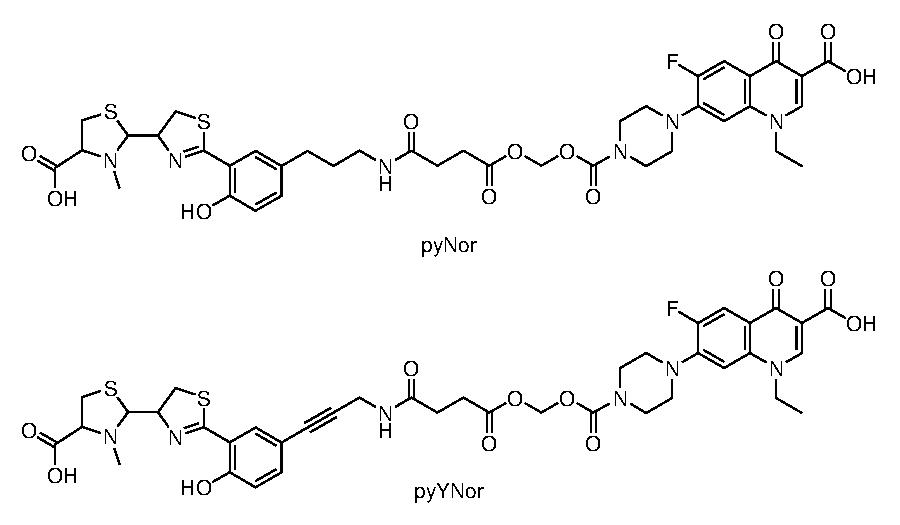
\includegraphics[scale=1]{pyNors}
		\caption{The cleavable pyochelin–norfloxacin conjugates synthesised by Rivault \textit{et al.}\cite{Rivault2007}. \label{fgr:pyNors}}
	\end{center}
\end{figure}

The properties of similar linkers (see \ref{fgr:cleavable_general}, R = Me) were studied by Gogate \textit{et al.}, who found that they were stable for more than 3 years under optimal conditions\cite{Gogate1987}. 
The hydrolysis of a secondary amine prodrug is dependent on ester hydrolysis rate, therefore the cleavage rate can be tuned by changing the R group between the ester and amide\cite{Ortmann2005}. 
The \textit{N}-(acetoxyethoxycarbonyl) (R = Me) linkers have been shown to be cleaved by esterases at an enhanced rate compared to buffer, and thus show promise in prodrugs\cite{Gogate1987a}. It was therefore hoped that they will allow intracellular release of the ciprofloxacin \compound{cmpd:Cip} payload from the conjugates in this study. Both the \textit{N}-(acetoxymethoxycarbonyl) (R = H) and \textit{N}-(acetoxyethoxycarbonyl) (R = Me) were used, to investigate whether differences in cleavage rate could tune activity.

\begin{figure}[H]
	\begin{center}
		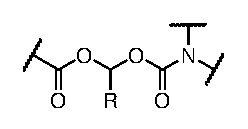
\includegraphics[scale=1]{cleavable_general}
		\caption{The cleavable linkers investigated in this study. \label{fgr:cleavable_general}}
	\end{center}
\end{figure}

\subsubsection{HSL analogue-ciprofloxacin conjugates\label{sec:AIA_intro}}

Following on from the library of compounds based on \textit{P. aeruginosa} autoinducers, a series of conjugates based on \textit{analogues} of HSL were planned. This strategy was inspired by a paper\cite{Ganguly2011} and patent\cite{Iyer2012} by Ganguly \textit{et al.}, who synthesised and characterised a conjugate \compound{cmpd:SHL4CipMe} of methyl ciprofloxacin with homocysteine thiolactone (see \ref{fgr:SHL4CipMe}). Homocysteine thiolactone is an analogue of homoserine lactone with the ring oxygen replaced by sulfur, and has been used as the head group in several other known quorum sensing modulators\cite{Eberhard1986,Schaefer1996,Passador1996,Smith2003,Chhabra1993,McInnis2011,Geske2007,Janssens2007}.


\begin{figure}[H]
	\begin{center}
		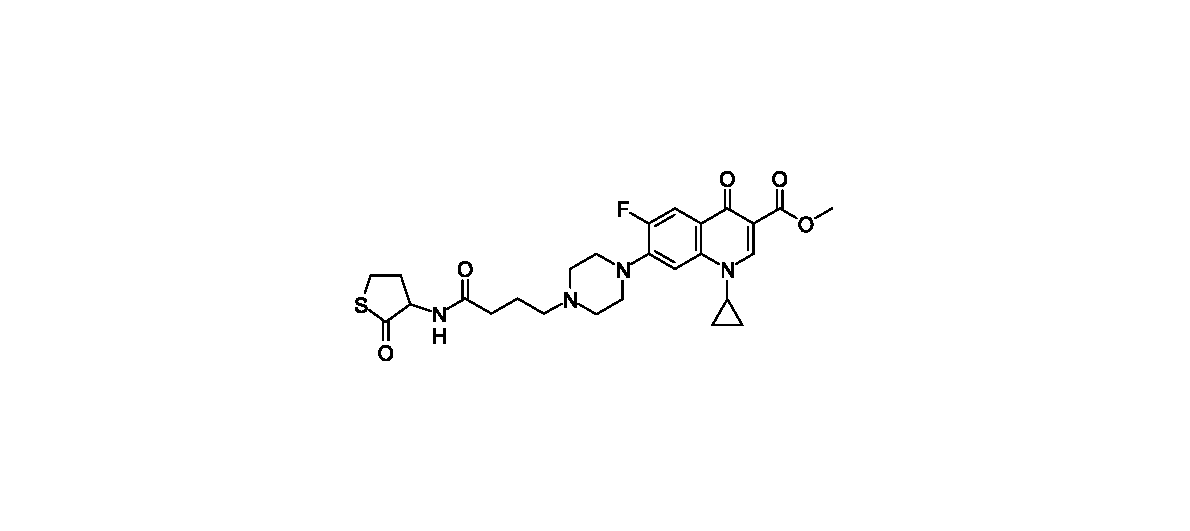
\includegraphics[scale=1]{SHL4CipMe}
		\caption{The HCTL-CipMe conjugate \compound{cmpd:SHL4CipMe} studied by Ganguly \textit{et al.}\cite{Ganguly2011,Iyer2012}.\label{fgr:SHL4CipMe}}
	\end{center}
\end{figure}


As part of their characterisation of the HCTL-CipMe conjugate \compound{cmpd:SHL4CipMe}, Ganguly \textit{et al.} found the minimum inhibitory concentration (MIC) of the conjugate in \textit{P. aeruginosa} under standard planktonic conditions. 
The MIC was found to be ten times higher for the conjugate vs. ciprofloxacin (50 vs. 5 $\mu$m), indicating that the conjgate was less effective than ciprofloxacin under planktonic conditions. 

Ganguly \textit{et al.} then investigated the effect of the conjugate on biofilms. 
The conjugate and ciprofloxacin were first added to dilute \textit{P. aeruginosa} liquid culture at 25 $\mu$m. 
As expected, the culture failed to grow and form biofilm in the presence of ciprofloxacin, but did grow in the presence of the conjugate \compound{cmpd:SHL4CipMe}. 
They then incubated cultures for 24 h, to allow biofilms to grow, before adding the compounds. In contrast, they found that the conjugate \compound{cmpd:SHL4CipMe} disrupted the biofilm more effectively than ciprofloxacin. 
When the biofilm was grown for 48 or 72 hours the conjugate had similarly disruptive effects, whereas ciprofloxacin `did not show any significant antibacterial activity'.

These results are exciting as they hint that an autoinducer conjugate might be able to combat an established \textit{P. aeruginosa} infection more effectively than the unmodified antibiotic. 
Ganguly \textit{et al.} suggest that their conjugate is more effective than ciprofloxacin in penetrating biofilms, and/or better at avoiding being pumped out by multidrug efflux pumps. They posit that this could be due to the thiolactone head, as they also showed that unconjugated C$_4$-HCTL \compound{cmpd:SHL4} (see \ref{fgr:HL_SHL}) has `either enhanced uptake or functional activity' when compared with C$_4$-HSL \compound{cmpd:HL4}. 

It is possible that the conjugate \compound{cmpd:SHL4CipMe} has higher activity against biofilms when compared with ciprofloxacin \compound{cmpd:Cip} because conjugate \compound{cmpd:SHL4CipMe} avoids being pumped out by multidrug efflux pumps, or selects for the survival of mutants with upregulated efflux pumps, and hence disrupted quorum sensing systems (see \ref{sec:conj_eff}).

While one might expect the conjugate \compound{cmpd:SHL4CipMe} to behave like C$_4$-HSL \compound{cmpd:HL4}, and hence passively diffuse in and out of cells, it is possible that its transport more closely resembles that of 3-oxo-C$_{12}$-HSL \compound{cmpd:HLO12}. 3-oxo-C$_{12}$-HSL \compound{cmpd:HLO12}'s accumulation in membranes and interaction with efflux pumps is thought to be based primarily on tail chain length (see \ref{sec:AI_eff}), and the ciprofloxacin half of the conjugate \compound{cmpd:SHL4CipMe} could be seen as a long tail, especially as the carboxylic acid is methylated and hence less polar.

\begin{figure}[H]
	\begin{center}
		\schemeref[HL4]{cmpd:HL4}
		\schemeref[SHL4]{cmpd:SHL4}
		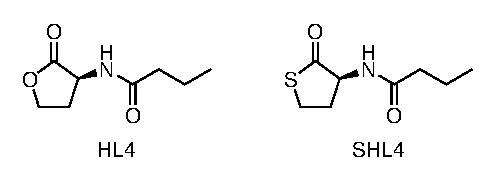
\includegraphics[scale=1]{HL_SHL}
		\caption{
		C$_4$-HSL \compound{cmpd:HL4} and C$_4$-HCTL \compound{cmpd:SHL4}. Note that Ganguly \textit{et al.} tested the \textit{S} enantiomer of C$_4$-HCTL \compound{cmpd:SHL4}, but used a racemic mixture in their HCTL-CipMe conjugate. %Ikeda2001
		\label{fgr:HL_SHL}}
	\end{center}
\end{figure}

While the results found by Ganguly \textit{et al.} show promise, they only test one conjugate, and do not include controls to show that the HCTL group specifically is necessary for the enhanced effect.
It was therefore decided to build on this work by synthesising a series of ciprofloxacin conjugates with head groups taken from known quorum sensing modulators\cite{Galloway2011,Hodgkinson2012a}, a selection of which are described in \ref{tbl:head_groups}. 


\begin{table}[H]
  \centering
\begin{tabular}{|P{0.18\textwidth}|p{0.32\textwidth}|p{0.32\textwidth}|}
\hline 
 \vspace{8px}\textbf{Head group} & \vspace{0px}\centering
\includegraphics[scale=1]{C4_tail} & \centering\arraybackslash\vspace{0px}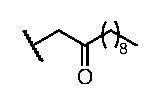
\includegraphics[scale=1]{oddhl_tail} \\ 
\hline 
 \vspace{0px}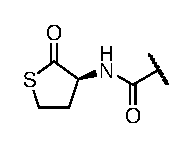
\includegraphics[scale=1]{SHL_head} & Partial agonist and antagonist against LasR\cite{McInnis2011}. Shown to increase biofilm formation in \textit{P. aeruginosa}\cite{Ganguly2011}.
 & Strong agonist against LasR, with comparable activity to the native ligand\cite{Smith2003,Boursier2018,Passador1996,McInnis2011}. \\ 
 %L vs racemate doesn't matter \cite{McInnis2011} D might actually do better?
 %check receptor. hydrolytic stability is higher for SHL. is it racemic in Ganguly?
 %Some evidence that \textit{R} enantiomer is more potent\cite{McInnis2011}.
%\hline 
% \vspace{0px}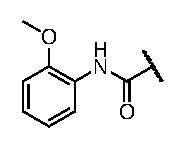
\includegraphics[scale=1]{2MeOA_head} 
% & Not yet studied. 
% & Not yet studied. \\  
\hline 
 \vspace{0px}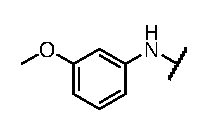
\includegraphics[scale=1]{3MeOA_head} 
 & Partial agonist against LasR\cite{Hodgkinson2012a}. 
 & Strong antagonist against LasR\cite{Hodgkinson2012a}. \\ 
\hline 
 \vspace{0px}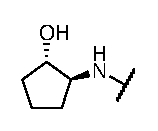
\includegraphics[scale=1]{HOcy5_head} 
 & Poor agonist and antagonist against RhlR\cite{Smith2003a,Jog2006}.
 & Strong antagonist against LasR\cite{Smith2003a}.\\ 
\hline 
 \vspace{0px}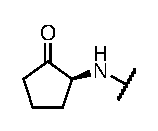
\includegraphics[scale=1]{Ocy5_head} 
 & Strong agonist against RhlR\cite{Smith2003a}. \textit{SS} enantiomer is more potent\cite{Jog2006}.
 & Partial agonist against LasR\cite{Smith2003a}. \\ 
\hline 
 \vspace{0px}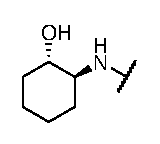
\includegraphics[scale=1]{HOcy6_head} 
 & Strong agonist against RhlR\cite{Smith2003a}. \textit{SS} enantiomer is more potent, with comparable activity to the native ligand\cite{Jog2006}.
 & Strong agonist against LasR\cite{Smith2003,Smith2003a}. \textit{SS} enantiomer is more potent, with comparable activity to the native ligand\cite{Jog2006}.\\ 
\hline 
 \vspace{0px}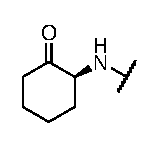
\includegraphics[scale=1]{Ocy6_head} 
 & Strong agonist against RhlR\cite{Smith2003a}. \textit{SS} enantiomer is more potent\cite{Jog2006}.
 & Partial antagonist against LasR\cite{Smith2003a}. Shown to reduce biofilm formation in \textit{P. aeruginosa}\cite{Smith2003a}.\\ 
\hline 
\end{tabular}
\caption{Activities of quorum sensing modulators containing the head groups used in this study.\label{tbl:head_groups}} 
\end{table}

\newpage

\section{Project aims and summary}

The aim of this project is to produce and test a library of autoinducer-antibiotic conjugates with the hope of producing conjugates with greater potency than the parent antibiotics.
The work is divided into two main sections. Section \ref{sec:AACs} focuses on conjugates of three \textit{P. aeruginosa} autoinducers (see \ref{fgr:PA_autoinducers}) with ciprofloxacin and trimethoprim (see \ref{fgr:ABs}) joined using a copper(I)-catalyzed azide-alkyne cycloaddition.
Section \ref{sec:HSLCipCs} focuses on conjugates of homoserine lactone analogues with ciprofloxacin (see \ref{sec:AIA_intro}) joined either using a copper(I)-catalyzed azide-alkyne cycloaddition or an S$_N$2 reaction or peptide coupling.






%The formation of biofilms can drastically increase MIC for many antibiotics \cite{Ceri1999}. For ciprofloxacin in \textit{P. aeruginosa} the MIC increases by 16 fold according to Ceri \textit{et al.} 

%Ganguly \textit{et al.} used Bac-Light Live/Dead staining and confocal microscopy to image the biofilms, whereas so far I have used crystal violet staining. Crystal violet does not differentiate between live or dead cells, and so might not pick up on the antibacterial effects of compounds. However, their confocal microscopy results show a quantifiable decrease in biofilm thickness, and it may be possible to detect this using crystal violet.

%
%\newpage
%
%\section{Aims}
%
%The aim of this project is to produce a library of autoinducer-antibiotic conjugates with the hope of increasing the potency of the drugs and possibly restoring their antibacterial action against resistant strains. The library is built from a collection of \textit{P. aeruginosa} autoinducer derivatives with azide groups attached and a collection of antibiotics with alkyne groups attached. These collections will then be combined using a copper(I)-catalysed azide-alkyne cycloaddition\cite{Tornoe2002,Rostovtsev2002} reaction to form the library of final conjugates. This approach has recently been used by Zheng \textit{et al.}\cite{Zheng2014} to join the siderophore enterobactin \compound{cmpd:entero} (see \ref{fgr:Sids}) with ampicillin or amoxicillin (see \ref{fgr:pen_anas} in \ref{sec:Futpen}).
%
%\subsection{autoinducer-antibiotic conjugates}
%
%A copper(I)-catalysed azide-alkyne cycloaddition\cite{Tornoe2002,Rostovtsev2002}, commonly referred to as a click reaction although this is a more general term, will be used to join each combination of autoinducer and antibiotic together (see \ref{sch:QSAB_synth_overv}). This modular approach allows the library to be easily expanded by adding more QMSs or antibiotics, or indeed other groups such as siderophores, fluorescent or affinity tags, or resin beads. The library will then be screened for antibiotic activity against \textit{P. aeruginosa} and other pathogenic bacteria.
%
%\begin{scheme}[H]
%	\begin{center}
%		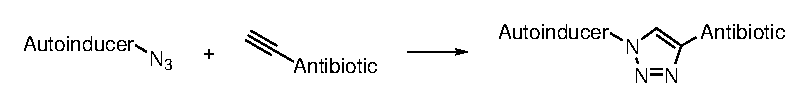
\includegraphics[scale=1]{QSAB_synth_overv}
%		\caption{The proposed construction of the library using a copper(I)-catalysed azide-alkyne cycloaddition. \label{sch:QSAB_synth_overv}}
%	\end{center}
%\end{scheme}
%
%\subsection{autoinducer derivatives}
%
%The four main autoinducers used by \textit{P. auruginosa} are shown in \ref{fgr:PA_autoinducers} in \ref{sec:PAautoinducers}. 
%We have decided to focus initially on the synthesis of azido analogues of C$_4$-HSL \compound{cmpd:HL4}, HHQ \compound{cmpd:HHQ} and PQS \compound{cmpd:PQS}. A synthesis of an azido analogue of 3-oxo-C$_{12}$-HSL \compound{cmpd:HLO12} has also been planned (see \ref{sch:HLO12N3_synth} in \ref{sec:Fut_HLO12}) and will be attempted in due course.
%
%The structure-activity relationships in PQS have been previously studied \cite{Hodgkinson2010}, and 5 and 6 positions could be substituted without significantly affecting the activity of the PQS molecule (see \ref{fgr:PQS_num}). Placing of the azide group at position 6 was chosen for synthetic reasons and the azide group was placed in the equivalent position in the HHQ analogue (see \ref{fgr:HHQPQSaz}).
%
%Alteration of the lactone group of C$_4$-HSL and other HSL derivatives is known to significantly decrease activity, especially where the number of H-bond donors or acceptors is altered \cite{Galloway2011}. Hence, the azide group will be included on the tail of C$_4$-HSL. Acyl tail length is known to play an important role in affinity, so we have decided to synthesise three analogues of C$_4$-HSL: azido-C$_2$-HSL \compound{cmpd:HL2N3}, azido-C$_4$-HSL \compound{cmpd:HL4N3} and azido-C$_6$-HSL \compound{cmpd:HL6N3} (see \ref{fgr:HL_anas}).
%
%
%
%\begin{figure}[H]
%	\begin{center}
%		\schemeref[PQS]{cmpd:PQS}
%		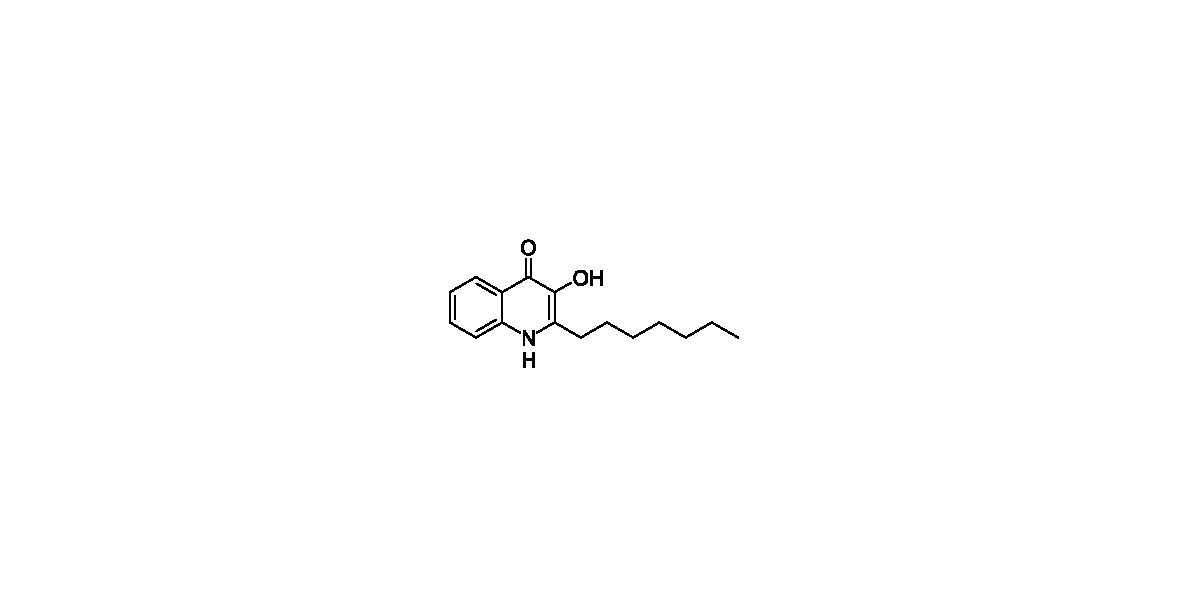
\includegraphics[scale=1]{PQS_num}
%		\caption{The atom numbering in PQS \compound{cmpd:PQS}. \label{fgr:PQS_num}}
%	\end{center}
%\end{figure}
%
%\begin{figure}[H]
%	\begin{center}
%		\schemeref[azHHQ]{cmpd:azHHQ}
%		\schemeref[azPQS]{cmpd:azPQS}
%		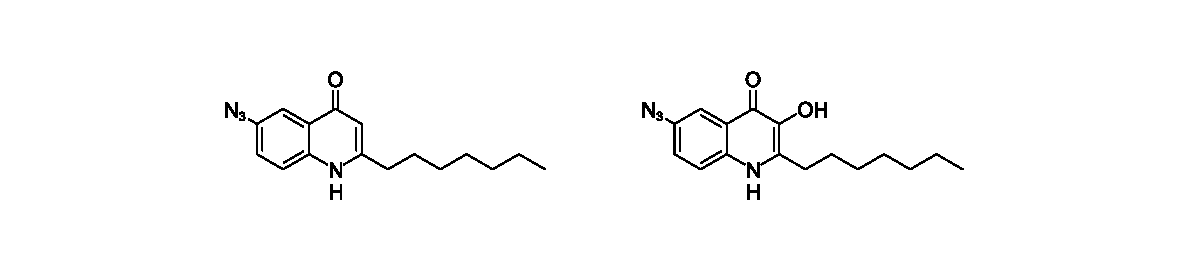
\includegraphics[scale=1]{azHHQPQS}
%		\caption{The HHQ \compound{cmpd:HHQ} and PQS \compound{cmpd:PQS} analogues \compound{cmpd:azHHQ} and \compound{cmpd:azPQS}. \label{fgr:azHHQPQS}}
%	\end{center}
%\end{figure}
%
%\begin{figure}[H]
%	\begin{center}
%		\schemeref[HL2N3]{cmpd:HL2N3}
%		\schemeref[HL4N3]{cmpd:HL4N3}
%		\schemeref[HL6N3]{cmpd:HL6N3}
%		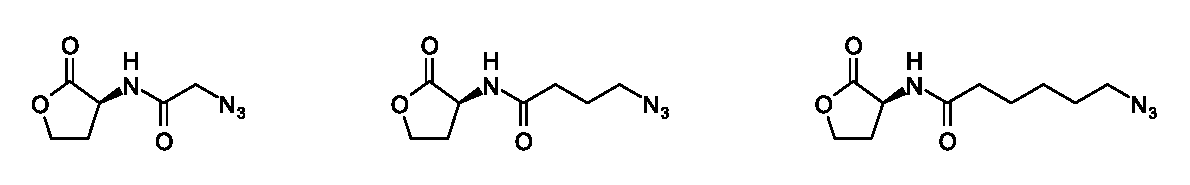
\includegraphics[scale=1]{HL_anas}
%		\caption{The C$_4$-HSL \compound{cmpd:HL4} analogues \compound{cmpd:cmpd:HL2N3}, \compound{cmpd:cmpd:HL4N3} and \compound{cmpd:cmpd:HL6N3}. \label{fgr:HL_anas}}
%	\end{center}
%\end{figure}
%
%\subsection{Ciprofloxcin analogues}
%
%Ciprofloxacin \compound{cmpd:cip} (see \ref{fgr:cip_num}) is second-generation fluoroquinolone antibiotic used to treat both Gram-positive and Gram-negative bacterial infections\cite{Oliphant2002}.
%The structure-activity relationships for ciprofloxacin have been investigated \cite{Renau1996} and positions 2 and 7 were found not to cause loss of activity. It was therefore decided that alkyne tails would be added at these positions giving two analogues of ciprofloxacin, \compound{cmpd:hexpipcip} and \compound{cmpd:pipciphex} (see \ref{sch:cip_anas}).
%
%\begin{figure}[H]
%	\begin{center}
%		\schemeref[cip]{cmpd:cip}
%		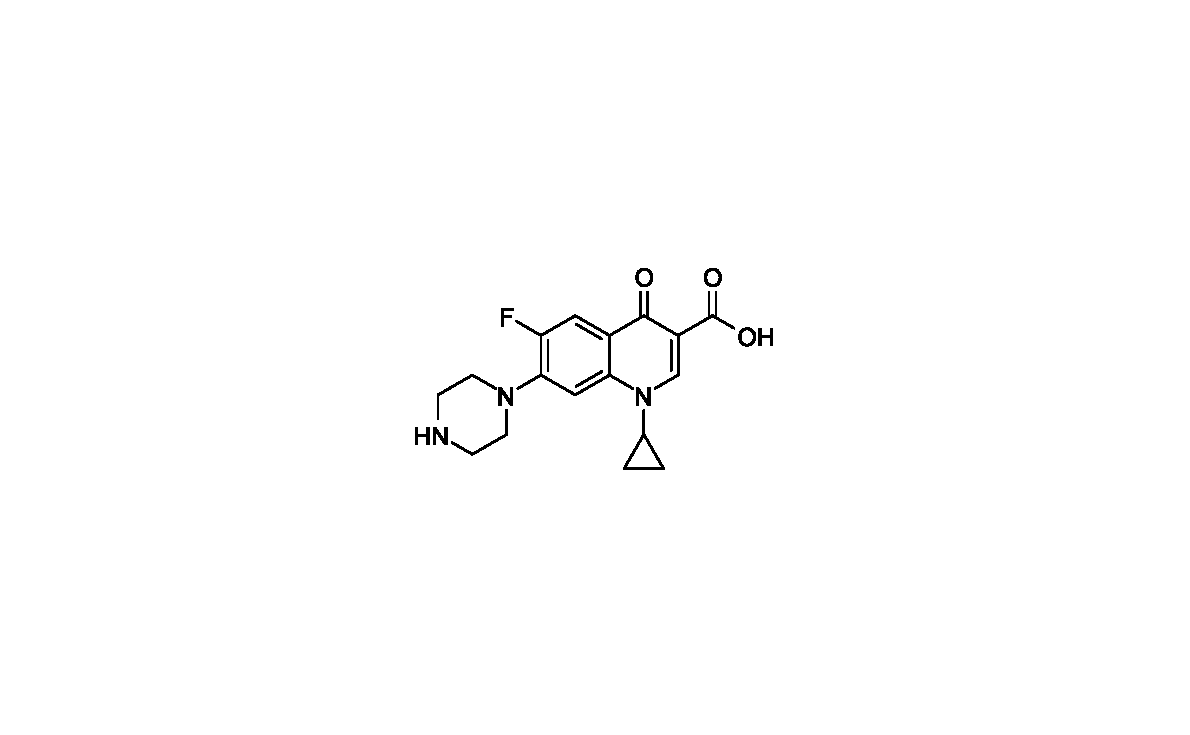
\includegraphics[scale=1]{cip_num}
%		\caption{The atom numbering in ciprofloxacin \compound{cmpd:cip}. \label{fgr:cip_num}}
%	\end{center}
%\end{figure}
%
%\begin{figure}[H]
%	\begin{center}
%		\schemeref[pipciphex]{cmpd:pipciphex}
%		\schemeref[hexpipcip]{cmpd:hexpipcip}
%		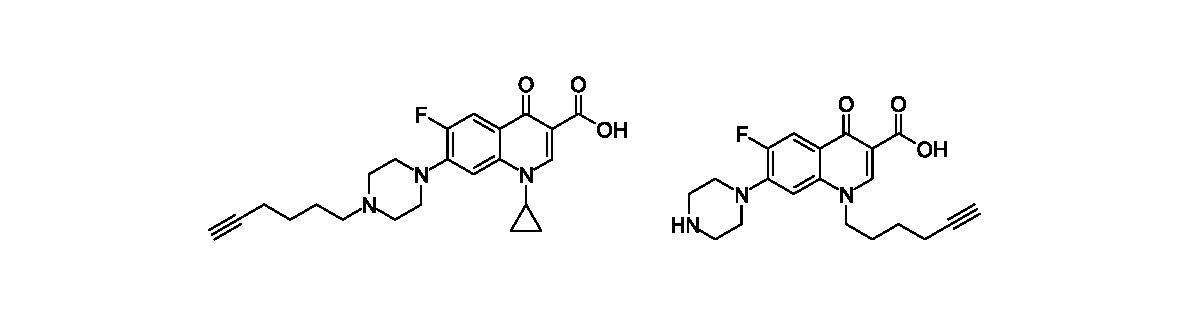
\includegraphics[scale=1]{cip_anas}
%		\caption{The proposed ciprofloxacin analogues \compound{cmpd:hexpipcip} and \compound{cmpd:pipciphex}. \label{sch:cip_anas}}
%	\end{center}
%\end{figure}
%
%, and this difference is more pronounced at high growth rates\cite{Evans1991}.
%In addition, the resistance of intact biofilms is significantly higher than that of resuspended biofilm cells, suggesting that organization of the cells within the biofilm confers resistance\cite{Evans1991}. 
%However, there are conflicting reports on whether \textit{P. aeruginosa} biofilms impede the diffusion of ciprofloxacin\cite{Suci1994,Shigeta1997,Kumon1994}, and regardless it has been shown that limited antibiotic diffusion through the biofilm is not the primary mechanism of resistance of \textit{P. aeruginosa} biofilms against ciprofloxacin \compound{cmpd:Cip}\cite{Walters2003}.
%Instead it is likely that poor oxygen penetration and low metabolic activity within the interior of the biofilm is responsible for the low antibiotic activity.
%This is expected for ciprofloxacin \compound{cmpd:Cip}, as it works by inhibiting DNA gyrase and topoisomerase IV, thereby inhibiting cell division.